\section{Case Study}
%This section highlights how the system helps analyze large text streams by applying it to the news dataset \emph{B} (Section~\ref{sec:results}).
%This section highlights the system \kg{analysis of} large text streams \kg{applied} to the news dataset \emph{B} (Section~\ref{sec:results}).
%\kg{In this section, we demonstrate the usage scenarios of our approach in real-world news/Twitter datasets.}
In this section, we demonstrate the usage scenarios of our approach \dc{using} real-world datasets.


%, Obama data.
%444,432 news articles that contain the keyword ``Obama,'' were collected from Sep. 1, 2012 to Jan. 14, 2013.
%Grouped by week, the articles were organized into 18 topic trees. %(Fig.~\ref{fig:obamatree}).
%%The average number of the first level nodes is 41, and the tree depth is 5($\pm 1$).
%The tree depths varied from 4 to 5, the total node numbers changed from 144 to 297, and the node
%number of the first level ranged from 18 to 79.
%\begin{figure}[ht]
%  \centering
%  \includegraphics[width=\columnwidth]{fig/obamatree}
%  \caption{Example topic tree for Obama data.}
%  \label{fig:obamatree}
%\end{figure}
\begin{figure*}[t]
\centering
%\vspace{-3mm}
\centering
  \includegraphics[width=\linewidth]{fig/Teaser}
    \vspace{-3mm}
  \caption{
%  \small
  %Overview of streaming hierarchical topics .
  %It provides an
%  Comparative analysis between the severity of epidemic and the intensity of public opinion in the Ebola dataset.
  Comparative analysis between the severity of \dc{the} epidemic and the intensity of public opinion in the Ebola dataset.
  %(a) Before Sep. 27, the most severe region, Africa, is the key focus of the public opinion.
  (a)  \kg{The region with the most severe cases (i.e., Africa)} was the key focus of public opinion \kg{before Sep. 27, 2014}.
  %During this period, the severity of epidemic is consistent with the intensity of public opinion.
  \kg{Epidemic severity during this period} was consistent with \kg{public opinion intensity.}
  %(b) After Sep. 27, there is an explosive growth of public discussion on the non-Africa regions.
  %(b) An explosive growth of public discussion on non-African regions \kg{occurred after Sep. 27.}
  (b) An explosive growth of public discussion \docpr{in} non-African regions \kg{occurred after Sep. 27.}
  %During this period, the intensity of public opinion is different with the severity of epidemic.
  \kg{Public opinion intensity during this period was inconsistent with epidemic severity.}
  }
%\vspace{-4mm}
\label{fig:msoverview}
\vspace{-5mm}
\end{figure*}
\subsection{Ebola Data}

%Ebola is a disease of humans and other primates caused by ebolaviruses.
%The largest outbreak of Ebola is the ongoing epidemic in West Africa.
%By Mar. 31, 2015, this outbreak has 25,263 reported cases resulting in 10,477 deaths.
%\kg{As of} Mar. 31, 2015, this outbreak \kg{had} 25,263 reported cases \kg{that resulted} in 10,477 deaths.
%We conducted the case study with a professor (P2) majored in public opinion analysis on healthcare.
%\kg{The} case study \kg{was conducted} with a professor (P2) \kg{who} majored in public opinion analysis on healthcare.
\kg{The} case study \kg{was conducted} with a professor (P2) \kg{who} majored in public opinion analysis \dc{in} healthcare.
%This case study aims at illustrating how TopicStream helps the expert examine the relationship between the severity of epidemic and the intensity of public opinion.
%This case study aims \kg{to illustrate} how TopicStream helps the expert examine the relationship between the severity of \kg{an} epidemic and the intensity of public opinion.
In this case study, we illustrate how TopicStream helps an expert examine the relationship between the severity of an epidemic (e.g., Ebola) and the intensity of public opinion.
%The severity of epidemic is measured by the reported case and death counts.
%The severity of \kg{the} epidemic is measured by the reported \kg{number of cases} and \kg{deaths}.
The severity of \kg{the} epidemic \docpr{was} measured by the reported \kg{number of cases} and \kg{deaths}.
%The intensity of public opinion is represented by the number of news articles and tweets at that time step (the width of the topic stripe).
The intensity of public opinion \docpr{was} represented by the number of news articles and tweets at that time step (the width of the topic stripe).
A wider stripe indicated more intense public opinion (Fig.~\ref{fig:msoverview}).\looseness=-1
%\kg{Fig.~\ref{fig:msoverview} shows that a} wider stripe \kg{indicated the intenser} public opinion.
%Moreover, it also demonstrates the capability of our tool in facilitating the expert to discover the major causes and the government's guidance on the opinion development.
%Moreover, it also demonstrates the \kg{ability} of our tool \kg{to enable} the expert to discover the major causes \kg{of} and the \kg{government} guidance on opinion development.

%A dataset that contains both news articles and tweets is used, which is collected by using keyword ``Ebola.''
%A dataset that contains both news articles and tweets collected by using keyword ``Ebola'' \kg{was used} (Dataset A).
A dataset that contains both news articles and tweets collected by using \docpr{the} keyword ``Ebola'' \kg{was used} (Dataset A).
Table~\ref{table:ebola} shows the statistics of the dataset.
\begin{table}[h]

\vspace{-3mm}
    \vspace{1mm}

    \centering
    \scalebox{0.8}{

    \begin{tabular}{|c|c|c|c|c|c|}

    \hline
    %Data & Time span & N\_num & T\_num & Depth & I\_num \\
    Data & Time span & $N_{num}$ & $T_{num}$ & \xiting{$h$} & $I_{num}$ \\
    \hline
   \emph{Old} & 7/27/2014-9/27/2014 & 51,318 & 7,161 & 3-4 & 77-150\\
   \hline
    \emph{New} & 9/28/2014-2/21/2015 & 156,088 & 15,558,371 & 3-5 & 34-223\\
   \hline
    \end{tabular}
    }
%        \vspace{-2mm}
    \caption{
%    \small
%The statistics of the Ebola dataset.
\kg{Statistics} of the Ebola dataset. \xiting{Here $N_{num}$ denotes the number of news articles, $T_{num}$ represents the number of tweets, $h$ is the tree depth, and $I_{num}$ denotes the number of internal nodes in the tree.}
}
\vspace{-5mm}
    \label{table:ebola}
\end{table}



\noindent \textbf{\normalsize Spread of Ebola outbreak.}
We first provided the professor (P2) with an overview of the old Ebola data.
%\kg{P2 was first provided} with an overview of the old Ebola data.
%The old data (before Sep. 27, 2014) is shown in Fig.~\ref{fig:msoverview}(a).
The old data (before Sep. 27, 2014) is shown in Fig.~\ref{fig:msoverview}(a).
%The news articles from Sep. 28 to Oct. 4 come in a streaming way Fig.~\ref{fig:msoverview}(b).
The news articles from Sep. 28 to Oct. 4 \kg{appeared in a streaming manner, as shown in} Fig.~\ref{fig:msoverview}(b).
%Based on topic keywords and corresponding news articles in Fig.~\ref{fig:msoverview}(a), the professor immediately identified the major topics in the news stream.
\kg{Using} topic keywords and corresponding news articles in Fig.~\ref{fig:msoverview}(a), %\kg{P2} immediately identified the major topics in the news stream, which are encoded by blue, pink, and yellow colors.
\kg{P2} immediately identified the major topics in the news stream, which \docpr{were} encoded \docpr{as} blue, pink, and \docpr{yellow.}
As in~\cite{cui2014}, we used the mean-shift clustering algorithm to cluster the topic at the first level since it is the most abstract level and can represent the topic tree very well.
For each cluster, we chose the topic closest to the cluster center as one focus topic.
%In this dataset, three focus topics encoded by blue, pink, and yellow colors, are automatically extracted by this method.
%, including ``Ebola-infected aid workers'' (blue), ``Ebola outbreak in Africa'' (pink), and ``Ebola patients and suspects outside Africa'' (yellow).


%By examining the incoming news articles on the pink topic stripe, ``Ebola outbreak in Africa'' (Fig.~\ref{fig:msoverview}A), she found that the epidemic is very serious in Africa.
By examining the incoming news articles on the pink topic stripe, ``Ebola outbreak in Africa'' (Fig.~\ref{fig:msoverview}A), \kg{P2} found that the epidemic \kg{was extremely} serious in Africa.
%It not only has the high death number (``Ebola: Killer virus death toll passes 3,000,'' Fig.~\ref{fig:msoverview}A1), but also the rapid growth of infections.
%It not only has the high death number (``Ebola: Killer virus death toll passes 3,000,'' Fig.~\ref{fig:msoverview}A1), but also the rapid growth of infections.
%\kg{The epidemic caused a large number of deaths} (``Ebola: Killer virus death toll passes 3,000,'' Fig.~\ref{fig:msoverview}A1) \kg{and the} growth of infections \kg{was rapid}.
\kg{The epidemic caused a large number of deaths} (Fig.~\ref{fig:msoverview}A1) \kg{and the} \dc{spread} of infections \kg{was rapid}.
%For example, in the news article ``Ebola could hit up to 1.4 mln West Africans by January: U.S. CDC,'' it is said ``Reported cases in Liberia are doubling every 15 to 20 days, and those in Sierra Leone are doubling every 30 to 40 days'' (Fig.~\ref{fig:msoverview}A2).
%For example, news article ``CDC worst case scenario for Ebola: 1.4 million cases'' mentioned that reported cases in Liberia are doubling every 15 to 20 days and those in Sierra Leone are doubling every 30 to 40 days (Fig.~\ref{fig:msoverview}A2).
For example, \docpr{the} news article \docpr{entitled} ``CDC worst case scenario for Ebola: 1.4 million cases'' mentioned that reported cases in Liberia \docpr{were} doubling every 15 to 20 days and those in Sierra Leone \docpr{were} doubling every 30 to 40 days (Fig.~\ref{fig:msoverview}A2).
%The blue topic stripe containing keywords ``dr,'' ``sacra,'' etc. talks about ``Ebola-infected aid workers''.
The blue topic stripe \kg{contains} keywords ``dr,'' ``sacra,'' \kg{and} talks about ``Ebola-infected aid workers.''
%``sacra'' is the last name of one of the aid workers, Dr. Rick Sacra.
\kg{``Sacra''} is the last name of \kg{Dr. Rick Sacra}, one of the aid workers.
%By examining the news articles in the archive area (Fig.~\ref{fig:msoverview}B), professor P2 learned that there are two aid workers returned to the U.S. for the treatment (``Second American health worker with Ebola arrives in U.S.'').
By examining the news articles in the archive area (Fig.~\ref{fig:msoverview}B), \kg{P2} learned that two aid workers returned to the U.S. for \kg{treatment}.
% (``Second American health worker with Ebola arrives in U.S.'').
%The increased width in the stack area (Fig.~\ref{fig:msoverview}C) talked about their recovery (``2 American Ebola patients released from hospital'').
The increased width in the stack area (Fig.~\ref{fig:msoverview}C) \kg{discussed} their recovery.
% (``2 American Ebola patients released from hospital'').
%Fig.~\ref{fig:msoverview}D and Fig.~\ref{fig:msoverview}E in the river area are about the third and fourth infected aid workers.
%Figs.~\ref{fig:msoverview}D and \kg{\ref{fig:msoverview}E} in the river area are about the third and fourth infected aid workers.
Figs.~\ref{fig:msoverview}D and \kg{\ref{fig:msoverview}E} in the river area are \dc{related to} the third and fourth infected aid workers.
%From the above exploration, she concluded that there are several infected aid workers, however, the situation is not serious.
From the \kg{preceding} exploration, \kg{P2} concluded that several aid workers \kg{had been infected;} however, the situation \kg{was} not serious.
%From the word cloud ( Fig.~\ref{fig:msoverview}F ) of the yellow topic stripe, professor P2 observed keywords like ``suspected,'' ``tested,'' ``york,'' ``sinai'' etc.
%From the word cloud ( Fig.~\ref{fig:msoverview}F ) of the yellow topic stripe, \kg{P2} observed keywords \kg{such as} ``suspected,'' ``tested,'' ``york,'' ``sinai.''
%From the word cloud ( Fig.~\ref{fig:msoverview}F ) of the yellow topic stripe, \kg{P2} observed keywords \kg{such as} ``suspected,'' ``york,'' \dc{and} ``sinai.''
From keywords ``suspected,'' ``york,'' \dc{and} ``sinai'' in the word cloud of the yellow topic stripe (Fig.~\ref{fig:msoverview}F)),  
%She found this topic is about ``Ebola patients and suspects outside Africa.''
\kg{P2} concluded \kg{that} this topic \kg{was} about ``Ebola patients and suspects outside Africa.''
%After reading the corresponding news articles before before Sep. 27, she concluded that there are only several suspects outside Africa and the situation is not serious.
After reading the corresponding news articles before Sep. 27, \kg{P2} concluded that only \kg{a few} suspects \kg{were} outside Africa and the situation \kg{was} not serious.\looseness=-1

\begin{figure*}[t]
	\centering
	\vspace{-2mm}
	\centering
	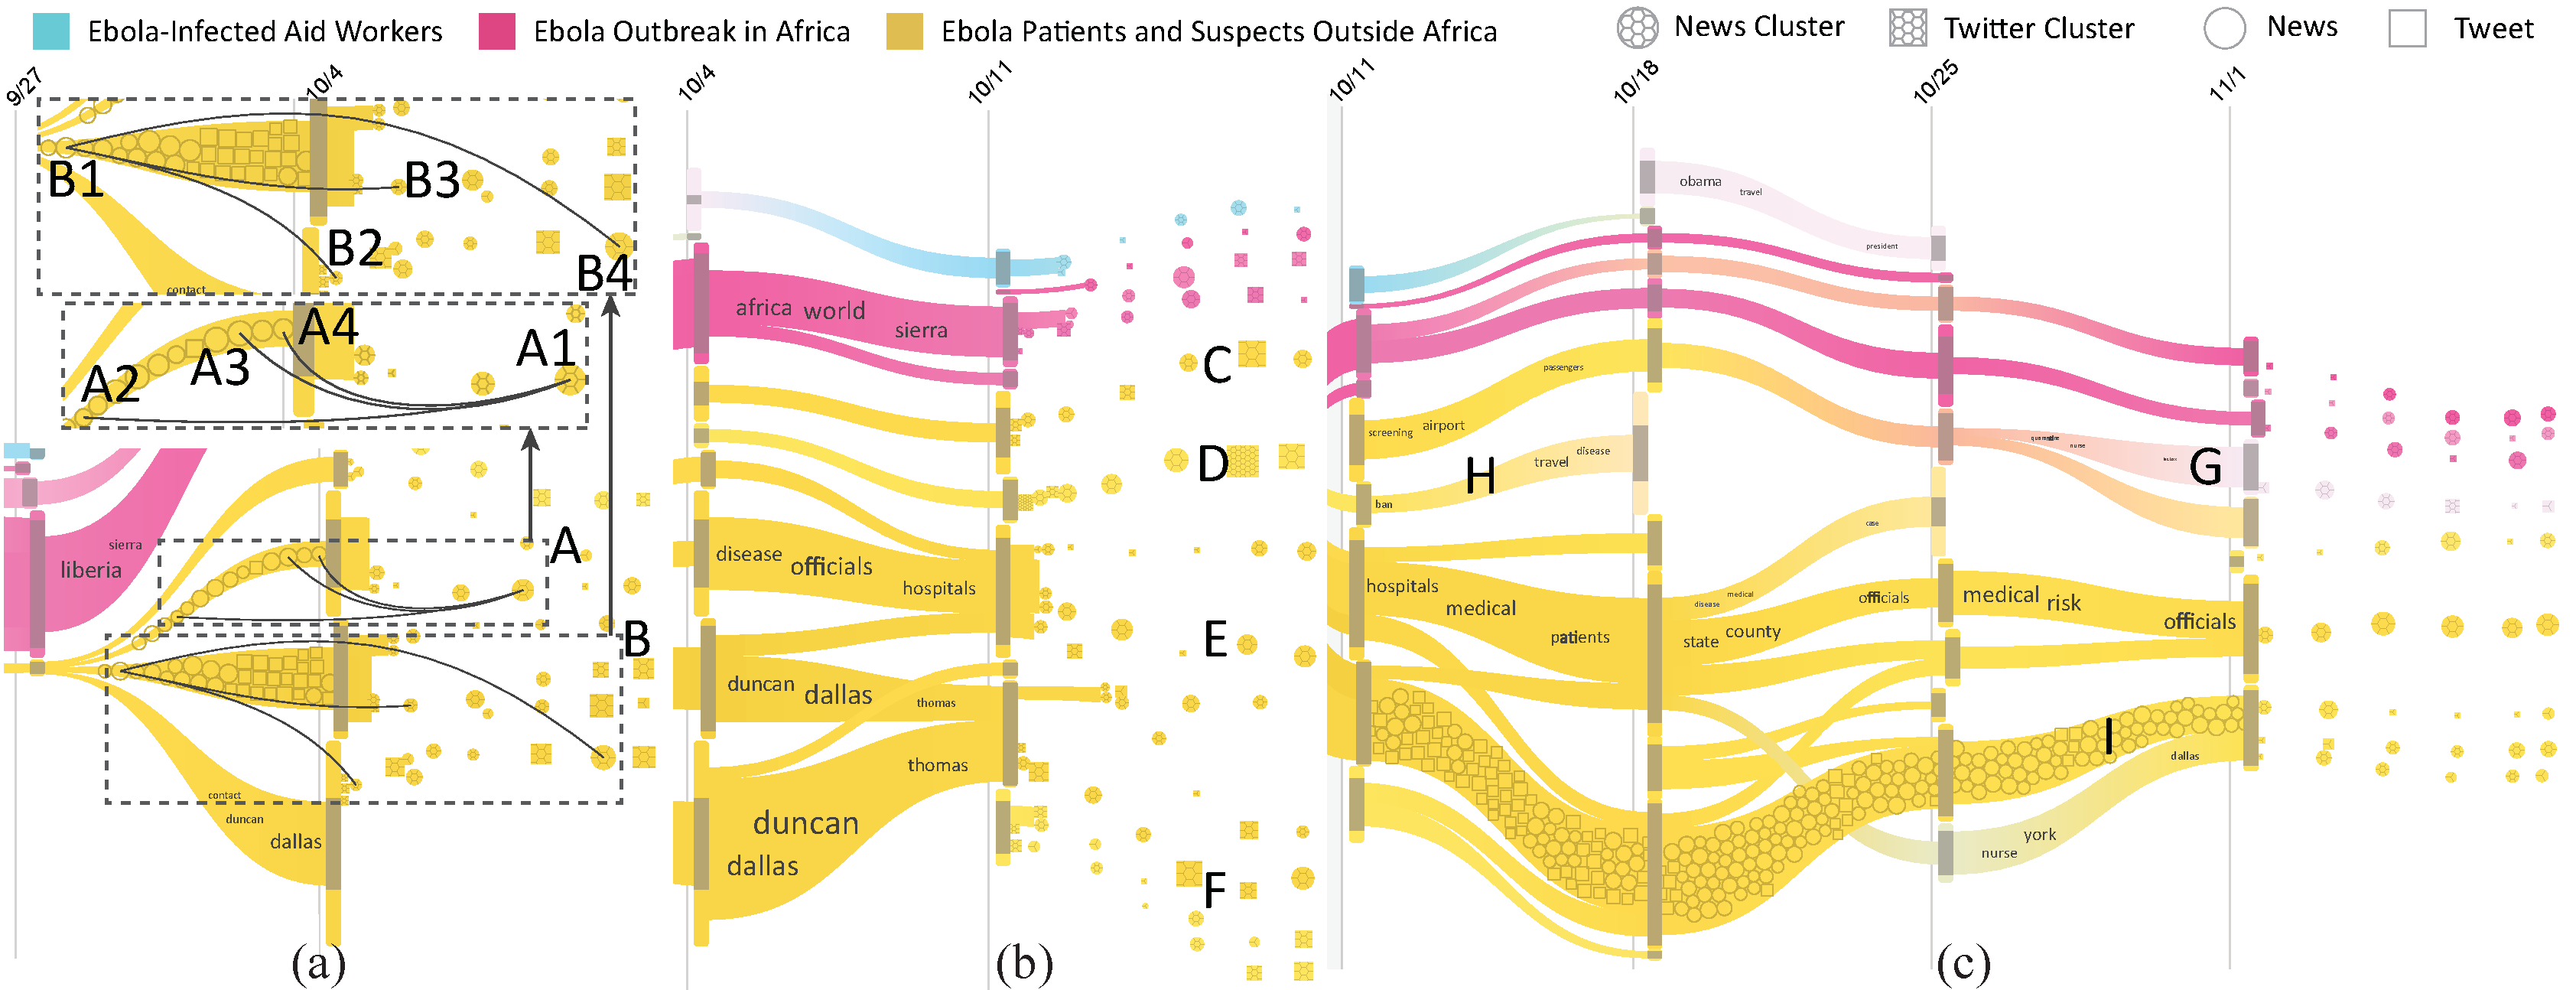
\includegraphics[width=\linewidth]{fig/ebola}
	\vspace{-3mm}
	\caption{
		%  \small
		%Explosive discussion on the the reported case outside Africa: (a) Oct. 5-11; (b) Oct. 12-18; (c) Nov. 2-8.
		%Explosive discussion on reported \kg{cases} outside Africa: (a) Oct. 5 to 11; (b) Oct. 12 to 18; (c) Nov. 2 to 8.
		Explosive discussion \docpr{of} reported \kg{cases} outside Africa: (a) Oct. 5 to 11; (b) Oct. 12 to 18; (c) Nov. 2 to 8.
	}
	\vspace{-5mm}
	\label{fig:ebola}
\end{figure*}

\noindent \textbf{\normalsize Explosive discussion on Ebola outside Africa.}
%Professor P2 found that the severity of epidemic is consistent with the intensity of public opinion before Sep. 27 (Fig.~\ref{fig:msoverview}(a)).
\kg{P2} found that the severity of \kg{the} epidemic \kg{was} consistent with the intensity of public opinion before Sep. 27 (Fig.~\ref{fig:msoverview}(a))\kg{,}
%Namely, the wider the stripe, the more intense the public opinion.
that is, the stripe \kg{was wider}, \kg{which indicated} more intense public opinion.
%However, after Sep. 28, there is an explosive discussion on Ebola outside Africa (Fig.~\ref{fig:msoverview}(b)).
However, as indicated by the increasing number of yellow circles and squares in the visualization (Fig.~\ref{fig:msoverview}(b)), there is an explosive discussion on Ebola outside Africa \kg{occurred} after Sep. 27.
%Professor P2 was curious about such a change, so she continued to explore the incoming data.
P2 was curious about such a change\kg{;} \kg{thus, the exploration of} the incoming data \kg{continued}.


%She noticed that the explosion began at the news cluster denoted by Fig.~\ref{fig:msoverview}G, which contains many news articles.
She noticed that the explosion began at the news cluster denoted by Fig.~\ref{fig:msoverview}G, which \kg{contained} many news articles.
The news cluster was then followed by several Twitter clusters.
%After some exploration, she found the news cluster is mainly about the first case of Ebola in the US (``CDC confirms first case of Ebola in US'').
After some exploration, \kg{P2} found \kg{that} the news cluster \kg{was} mainly about the first case of Ebola in the US.
 %(``CDC confirms first case of Ebola in US'').
%The patient, Thomas Duncan, had come into contact with as many as 80 people.
The patient, Thomas Duncan, had \kg{been exposed to} as many as 80 people.
%The first confirmation case led to a lot of discussion on Twitter (``....hmm Fwd: US Government Confirms an Ebola Case in Texas! http://t.co\/GNcFZGWzEz sponsor=femiolulana'') and created fears (``I don't even know what're symptoms are for Ebola But I think I got them'').
The first confirmed case led to \kg{numerous} discussion\kg{s} on Twitter
 %(``....hmm Fwd: US Government Confirms an Ebola Case in Texas! http://t.co\/GNcFZGWzEz sponsor=femiolulana'')
and created fear.
% (``I don't even know what're symptoms are for Ebola But I think I got them'').
%Because of the heightened attention from the public and media, this topic is divided into four sub-topics:
Because of the heightened attention from the public and media, this topic \docpr{was} divided into four sub-topics:
1) the further report of suspects (Fig.~\ref{fig:msoverview}H);
2) government actions (Fig.~\ref{fig:msoverview}I);
3) treatment of the patient (Fig.~\ref{fig:msoverview}J);
%and 4) search for people who had some form of contact with the patient (Fig.~\ref{fig:msoverview}K).
and 4) \docpr{the} search for people who had some form of contact with the patient (Fig.~\ref{fig:msoverview}K).\looseness=-1
%\kg{This} topic is divided into four sub-topics \kg{because of the heightened attention from the public and media.}
%\kg{The Topics are} 1) further report of suspects (Fig.~\ref{fig:msoverview}H); 2) \kg{government} actions (Fig.~\ref{fig:msoverview}I); 3) \kg{treatment} of the patient (Fig.~\ref{fig:msoverview}J); and 4) search \kg{for} people who \kg{had some form of} contact with the patient (Fig.~\ref{fig:msoverview}K).

%Professor P2 commented that the public and news media in the US did not pay too much attention to the Ebola epidemic when it happened in Africa (before Sep. 27) and observed it in the other's perspective.
%\kg{P2} commented that the public and news media in the US \kg{paid minimal} attention to the Ebola epidemic happened in Africa \kg{before Sep. 27, observing the epidemic from the other's perspective.}
%\kg{P2} commented that the public and news media in the US \kg{paid minimal} attention to the Ebola epidemic \dc{in} Africa \kg{before Sep. 27, observing the epidemic from the other's perspective.}
\kg{P2} commented that the public in the US \kg{paid minimal} attention to the Ebola epidemic \dc{in} Africa \kg{before Sep. 27, observing the epidemic from the other's perspective.}
This is consistent with the theory of alterity (otherness)~\cite{otherness}.
%consistent with the theory of alterity (otherness)~\cite{otherness}.
%It broke such a perspective when it happened around themselves and led to an intensive discussions on news media and Twitter.
%\kg{When the epidemic} happened \kg{in the US, the perspective changed} and led to intensive discussions on news media and Twitter.
\kg{When the epidemic} \dc{arrived} \kg{in the US, the perspective changed} and led to \dc{intense} discussions on news media and Twitter.
%She further explained the spread of the first case in the US also disclosed another phenomenon.
\kg{P2} further explained \kg{that} the spread of the first case in the US also disclosed another phenomenon.
%Since the news media reported the first case wantonly, the severity of the epidemic was overestimated and fears were created among average persons.
%Since the news media reported the first case wantonly, the severity of the epidemic was overestimated and fears were created among average \dc{people}.
Since the news media reported the first case wantonly, the severity of the epidemic was overestimated and \docpr{fear was} created among average \dc{people}.
%\kg{The} severity of the epidemic \kg{was} \kg{overestimated} and fears were created among average persons \kg{because the news media reported the first case wantonly and because}
%This is due to that the human perceptual world is often influenced by the pseudo society built by the media.
This is \dc{because human perception} is often influenced by the pseudo society built by the media.
%the \kg{human} perceptual world is often influenced by the pseudo society built by the media.
%Under such situation, it is very important for the government to take actions to guide the public opinion.
Under such \kg{a} situation, the government \kg{must} guide public opinion.

%\noindent \textbf{Government's action and guidance.}
\noindent \textbf{\normalsize \kg{Action} and guidance \kg{of the government}.}
%Professor P2 wanted to know the US government's actions on the epidemic.
%Thus she continued examining more new documents.
%\kg{P2} continued examining new documents \kg{to know the actions of the US government on the epidemic}.
\kg{P2} continued examining new documents to \dc{learn} the actions of the government \dc{regarding} the epidemic.
%She found there was few discussion on Twitter on topic ``government's actions'' from Oct. 5 to Oct. 11 (Fig.~\ref{fig:ebola}A).
%She found few discussion on Twitter on topic ``\dc{government actions}'' from Oct. 5 to Oct. 11 (Fig.~\ref{fig:ebola}A)\kg{,}
%She found few \dc{discussions} on Twitter on topic ``\dc{government actions}'' from Oct. 5 to Oct. 11 (Fig.~\ref{fig:ebola}A)\kg{,}
She found few \dc{discussions} on Twitter on \docpr{the} topic ``\dc{government actions}'' from Oct. 5 to Oct. 11 (Fig.~\ref{fig:ebola}A)\kg{,}
%This indicates that this topic does not attract too much attention from the public.
\kg{indicating} that this topic \kg{failed to} attract \kg{public} attention.
%On the contrary, there was a lot of discussion on Twitter on the death of the Ebola patient (Fig.~\ref{fig:ebola}B).
On the contrary, \kg{numerous discussions} on Twitter \kg{focused} on the death of \kg{an} Ebola patient (Fig.~\ref{fig:ebola}B).\looseness=-1


%In order to figure out the reason, she examined these two topics in Fig.~\ref{fig:ebola}(a) and found one representative cluster (A1, ``CDC urges hospitals to follow Ebola-related protocols'') and document (B1, ``Dallas hospital isolating patient being tested for Ebola'').
\kg{To identify} the reason, \kg{P2} examined these two topics in Fig.~\ref{fig:ebola}(a) and found one representative cluster (Fig.~\ref{fig:ebola}A1, ``EbolaCDC urges hospitals to follow Ebola-related protocols'') and document (Fig.~\ref{fig:ebola}B1, ``Dallas hospital isolating patient being tested for Ebola'').
%She then explored their similar documents/clusters in the adjacent time points to know how the topics evolved in the stream.
%She then explored similar documents \kg{or} clusters in the adjacent time points to know \kg{the evolution of} the topics in the stream.
She then explored similar documents \kg{or} clusters in the adjacent time steps to \dc{determine} \kg{the evolution of} the topics in the stream.
%From the links and corresponding documents in Fig.~\ref{fig:ebola}A, she found the government immediately took actions and prepared for Ebola before Oct. 1: 1) Sep. 30, ``Health Ministry to distribute 10,000 PPEs on Thursday'' (A2); 2) Oct. 2, ``Local hospitals prepared in case of Ebola'' (A3); 3) Oct. 2, ``Ebola 'unlikely' but South prepared'' (A4).
From the links and corresponding documents in Fig.~\ref{fig:ebola}A, \kg{P2} found \kg{that} the government immediately took \kg{action} and prepared for Ebola before Oct. \kg{4}, \kg{as shown by the following news articles}: 1) Sep. 30, ``Health Ministry to distribute 10,000 PPEs on Thursday'' (Fig.~\ref{fig:ebola}A2); 2) Oct. 2, ``Local hospitals prepared in case of Ebola'' (Fig.~\ref{fig:ebola}A3); \kg{and} 3) Oct. 2, ``Ebola `unlikely' but South prepared'' (Fig.~\ref{fig:ebola}A4).
%From the links and corresponding clusters, the professor got the idea that the patient's condition was getting worse and finally died: 1) Oct. 5, ``Dallas Ebola patient is in critical condition, hospital say'' (B2); 2) Oct. 5, ``Ebola patient in Dallas 'took a turn for the worse'' (B3); 3) Oct. 8, ``Dallas Ebola Patient Dies'' (B4).
From the links and corresponding clusters in Fig.~\ref{fig:ebola}B, \kg{P2 realized} that the patient's condition \kg{worsened and led to death, as indicated by the following news articles}: 1) Oct. 5, ``Dallas Ebola patient is in critical condition, hospital says'' (Fig.~\ref{fig:ebola}B2); 2) Oct. 5, ``Ebola patient in Dallas takes a turn for worse'' (Fig.~\ref{fig:ebola}B3); \kg{and} 3) Oct. 8, ``Dallas Ebola Patient Dies'' (Fig.~\ref{fig:ebola}B4).
%The professor believed that the government took the right action in time.
\kg{P2} believed that the government acted promptly.
However, the death of the patient
%The key leading to the uncontrolled public opinion is the death of the patient.
\kg{led} to uncontrolled public opinion.

\begin{figure*}[t]
	\centering
	%\vspace{-3mm}
	\centering
	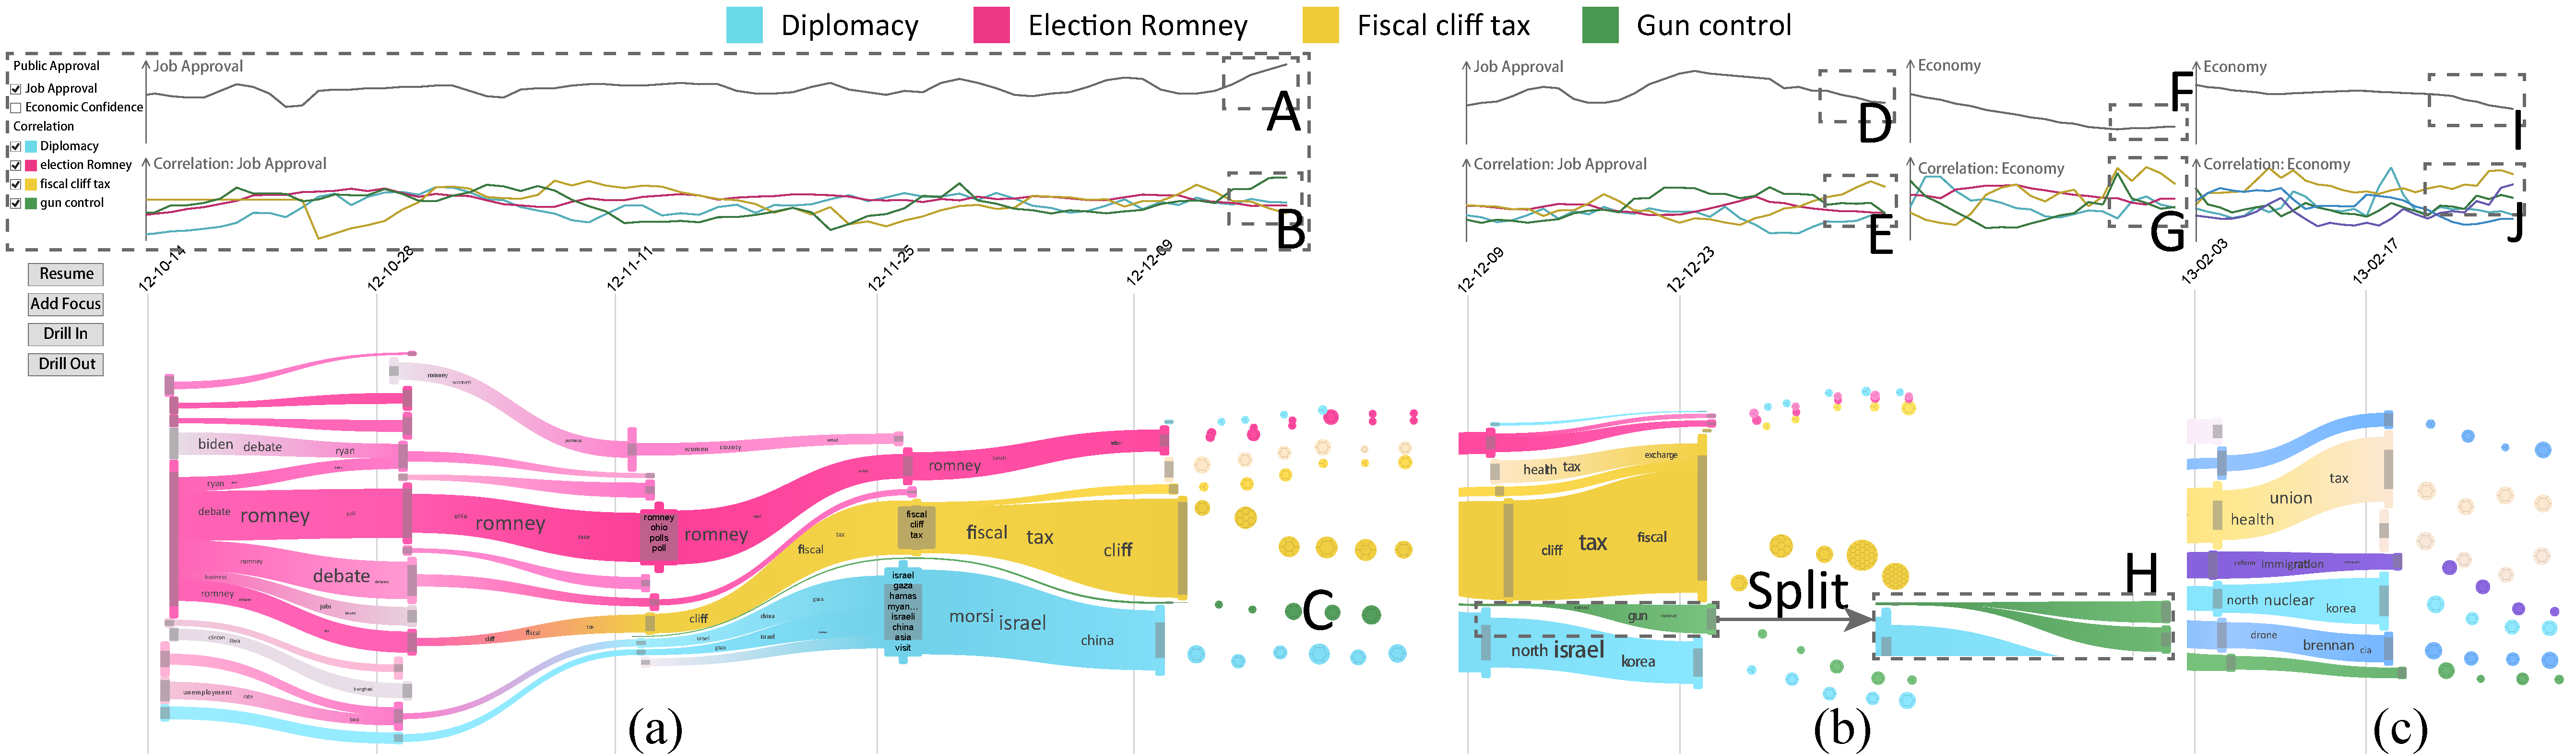
\includegraphics[width=\linewidth]{fig/obamacase1}
	\vspace{-4mm}
	\caption{
		Significant changes in public opinion in the Obama dataset.
		%Correlations are shown to help analyzing the reason for the changes.
		%(a) Presidential approval rate affected by topic ``Gun Control.''
		(a) Presidential approval \docpr{rating} affected by topic ``Gun Control.''
		%   The topic ``gun control'' (green) was triggered by a shooting accident.
		%   %Topic ``Gun Control'' (green) had a boost in the period of Obama's second term of office.
		%   Obama's response for this accident fit public opinion. This may be one leading factor of the increase of his job approval.
		%(b) A decrease of presidential approval and economic confidence caused by the fiscal cliff crisis.
		(b) A decrease \kg{in} presidential approval and economic confidence caused by the fiscal cliff crisis.
		%Public attention transited to topic ``Fiscal Cliff.”
		%Public attention transferred to ``fiscal cliff". Obama's mistakes in handling the crisis caused critics to him and the crisis led to low economic confidence.
		%(c) Another low economic confidence caused by failed negotiation on spending cuts of the government.
		%(c) Another low economic confidence \kg{rating} caused by failed negotiation\kg{s} on spending cuts of the government.
		(c) Another low economic confidence \kg{rating} caused by failed negotiation\kg{s} on \docpr{government spending cuts}.
		%Initial layout of media topics related to ``Obama", public approval line and their correlation. Topics with high correlation or topic transition caused change in public approval.
		%High correlation between the yellow topic and the economic approval and Obama's failure on handling the economic crisis caused the .
	}
	\vspace{-5mm}
	\label{fig:obamacase1}
\end{figure*}


%Next, the documents in the week of Oct. 11 streamed in.
\kg{The} documents \kg{that subsequently streamed in were from} the week of Oct. 11.
%As shown in Fig.~\ref{fig:ebola}(b), public attention on topic ``government's action'' kept on decreasing (E).
%As shown in Fig.~\ref{fig:ebola}(b), public attention on  topic ``\dc{government action}'' \kg{decreased} (Fig.~\ref{fig:ebola}E)\kg{, whereas}
As shown in Fig.~\ref{fig:ebola}(b), public attention \docpr{to the}  topic ``\dc{government action}'' \kg{decreased} (Fig.~\ref{fig:ebola}E)\kg{, whereas}
%While there is increasing discussions on Twitter on topics ``airport screening'' (C, ``Ebola Screenings Begin at US Airports''), ``travel ban'' (D, ``RT @CronkiteSays: VIEWER POLL\#N\#Do you support a travel ban from Ebola inflicted countries?''), and ``infected nurse'' (F, ``Dallas Nurse With Ebola Identified'').
discussions on Twitter on topics ``airport screening'' (Fig.~\ref{fig:ebola}C, ``Ebola Screenings Begin at US Airports''), ``travel ban'' (Fig.~\ref{fig:ebola}D, ``RT @CronkiteSays: VIEWER POLL\#N\#Do you support a travel ban from Ebola inflicted countries?''), and ``infected nurse'' (Fig.~\ref{fig:ebola}F, ``Dallas Nurse With Ebola Identified'') \kg{increased}.
%The public pay further attention to negative messages.
%The public \kg{paid} further attention to negative messages.
The public \kg{paid} \dc{more} attention to negative messages.
%The situation was improved after three weeks (Fig.~\ref{fig:ebola}(c)).
The situation \dc{improved} after three weeks (Fig.~\ref{fig:ebola}(c)).
%The professor analyzed the documents and concluded three reasons for this change.
\kg{P2} analyzed the documents and \kg{specified} three reasons for this change.
%First, the evolvement of ``airport screening'' into another new topic shifted the public attention (F).
%First, the \kg{change} of ``airport screening'' into another new topic shifted the public attention (\kg{G}).
First, the \kg{change} \dc{from topic} ``airport screening'' \dc{to} another \dc{topic} shifted \dc{public attention} (\kg{Fig.~\ref{fig:ebola}G}).
%The new topic is relevant to quarantine, whose birth is caused by nurse Kaci Hickox defied the state's quarantine after she returned from treating Ebola patients in West Africa.
%The new topic \kg{was} relevant to quarantine, \kg{which emerged because of} nurse Kaci Hickox \kg{who} defied the quarantine \kg{imposed on her} after \kg{returning} from treating Ebola patients in West Africa.
The new topic \kg{was} \dc{related} to quarantine, \kg{which emerged because} nurse Kaci Hickox \dc{defied} the quarantine \kg{imposed on her} after \kg{returning} from treating Ebola patients in West Africa.
%This event caused a great disturbance and shifted the public attention.
%This event caused great disturbance and shifted the public attention.
This event caused great disturbance and \docpr{shifted public} attention.
%Second, topic ``travel ban'' gradually died after president Obama decided to cancel the travel ban (H).
%Second, topic ``travel ban'' gradually \kg{disappeared} after \kg{President} Obama decided to cancel the travel ban (H).
Second, topic ``travel ban'' gradually \kg{disappeared} after \kg{President} Obama decided to cancel the travel ban (Fig.~\ref{fig:ebola}H).
%Third, the popularity of ``infected nurse'' gradually decreased as the nurse was cured and got back to normal life(I, ``Amber Vinson, Dallas nurse, leaving hospital after Ebola cure'').
Third, the popularity of ``infected nurse'' gradually decreased as the nurse was cured and \kg{returned} to normal life (Fig.~\ref{fig:ebola}I).
%, ``Amber Vinson, Dallas nurse, leaving hospital after Ebola cure'').
%By now, the fears caused by the first case of Ebola in the US disappeared and the government finally guided the public opinion to the right direction.
%By now, the fears caused by the first case of Ebola in the US disappeared and the government finally influenced \dc{public opinion to} the positive.
By now, fear caused by the first case of Ebola in the US disappeared and the government finally influenced \dc{public opinion to} \docpr{be more} positive.
%The professor summarized that the government was very successful by using another topic (``quarantine'', G) to shift the public attention from the negative opinion caused by the the first case of Ebola.
% J and K don't apprear in the paper, should we delete them?
%\kg{P2} indicated that the government was \kg{highly} successful \kg{in} using another topic (``quarantine'', G) to shift the public attention \dc{away} from the negative opinion caused by the first \kg{Ebola} case \kg{in the US}.
\kg{P2} indicated that the government was successful \kg{in} using another topic (``quarantine'', Fig.~\ref{fig:ebola}G) to shift \dc{public attention} \dc{away} from the negative opinion caused by the first \kg{Ebola} case \kg{in the US}.\looseness=-1

\subsection{Obama data}


\begin{table}[b]
	
	\vspace{-3mm}

	%\vspace{1mm}
	\centering
	\scalebox{0.9}{
		\begin{tabular}{|c|c|c|c|c|}
			\hline
			%Data & Time span & N\_num & Depth & I\_num \\
			Data & Time span & $N_{num}$ & $h$ & $I_{num}$ \\
			\hline
			\emph{Old} & 10/14/2012-12/8/2012 & 47,963  & 4-10 & 267-376\\
			\hline
			\emph{New} & 12/9/2012-2/21/2015 & 495,151 & 7-11 & 246-471\\
			\hline
		\end{tabular}
	}
%	 \vspace{-2mm}
	\caption{
		%    \small
		%The statistics of the Obama dataset.
		\kg{Statistics} of Obama dataset.
	}
	\label{table:obama}	
\end{table}


%In the second case study, we collaborated with professor P1 in media and communication.
%The second case study was \kg{a collaboration} with a professor \kg{(}P1\kg{)} \kg{of} media and \dc{communication}.
The second case study was \kg{a collaboration} with a professor \kg{(}P1\kg{)} \kg{of} media and \docpr{communications}.
%He wanted to study the relationship between the media agenda (mass media) and public opinion,
In this case study, \kg{P1 studied} the relationship between the media agenda (mass media) and public opinion,
%which is a long-existing research topic in his field~\cite{McCombs1972}.
%a long-\kg{standing} research topic in \kg{the} field \kg{of media and communication}~\cite{McCombs1972}.
a long-\kg{standing} research topic in \kg{the} field of media and \dc{communication}~\cite{McCombs1972}.
%As public approval can be caused by compound factors, it's not intuitive to disclose the relationship between them.
%Thus he wanted to use our tool to help in the analysis.
%In addition this case study also shows the capability of our system to track the progress of an evolving event with the help of streaming visualization.
%He is particular interested in how sentiments of media agenda can affect public approval.

%We used a news dataset collected by using keyword ``Obama'' (dataset B), which is summarized in Table~\ref{table:obama}.
We used a news dataset collected by using \dc{the} keyword ``Obama'' \xiting{(Dataset B)}, which is summarized in Table~\ref{table:obama}.
%\kg{The} news dataset (\kg{the news dataset \emph{B}}) \kg{was} collected by using \kg{the} keyword ``Obama,'' \kg{as} summarized in Table~\ref{table:obama}.
%This professor's research interest is sentiment analysis on social media.
%As the cause of public approval is a long existing research topic in social science.
%to explore the news dataset \emph{B}.


%To analyze the correlation between the media agenda and public opinion, we added some contextual information (see the dashed rectangle in Fig.~\ref{fig:obamacase1}(a)).
%To analyze the \kg{relationship} between the media agenda and public opinion, we added some contextual information (see the dashed rectangle in Fig.~\ref{fig:obamacase1}(a)).
%To analyze the \kg{relationship} between the media agenda and public opinion, \kg{several} contextual information \kg{was added} (the dashed rectangle in Fig.~\ref{fig:obamacase1}(a)).
%To analyze the \kg{relationship} between the media agenda and public opinion, \kg{several} contextual information \dc{were} added (the dashed rectangle in Fig.~\ref{fig:obamacase1}(a)).
To analyze the \kg{relationship} between the media agenda and public opinion, \kg{several} \docpr{pieces of} contextual information \dc{were} added (the dashed rectangle in Fig.~\ref{fig:obamacase1}(a)).
%The contextual information consists of: 1) presidential approval rate of Obama and 2) economic confidence index derived from Gallup public opinion polls~\cite{Gallup}, as well as 3) the time varying statistical correlation between Gallup poll results and sentiment of media articles.
%The contextual information consists of: 1) \kg{Obama's} presidential approval \kg{rating}\kg{,} 2) \kg{an} economic confidence index derived from Gallup public opinion polls~\cite{Gallup}, \kg{and} 3) time\kg{-}varying statistical correlation between Gallup poll results and the sentiment of media articles.
The contextual information \dc{consists} of: 1) \kg{Obama's} presidential approval \kg{rating}\kg{,} 2) \kg{an} economic confidence index derived from Gallup public opinion polls~\cite{Gallup}, \kg{and}
%3) \dc{a} time\kg{-}varying statistical correlation between Gallup poll results and the sentiment of media articles.
3) \dc{a} time\kg{-}varying statistical correlation between \docpr{the} Gallup poll results and the sentiment of media articles.

%The public opinions were retrieved from Gallup website \cite{Gallup} (a leading company conducting public opinion polls).
A word-embedding-based sentiment classification algorithm~\cite{Tang2014} was employed to calculate the sentiment for each article.
%Each document was given a score from -1.0 to 1.0 where 1.0 means the most positive and -1.0 means the most negative.
%The topic sentiment at each time point is the average sentiments of the documents at that time point.
The topic \kg{``}sentiment\kg{''} at each time step \kg{refers to} the average sentiments of the documents at that time step.
%In our implementation, we calculate the sentiment every two weeks.
%We then obtained a sentiment time series for each topic.
\kg{A} sentiment time series \kg{was then obtained} for each topic.
Finally we calculated the Pearson correlation coefficient between a Gallup poll result and the temporal sentiment of a topic.\looseness=-1
%\kg{Finally,} the Pearson correlation coefficient \kg{was calculated} between a Gallup poll result and the temporal sentiment of a topic.
%In our experiment the window size was set to 14 days.

%\noindent \textbf{Presidential approval rate affected by topic ``Gun Control.'' }
%\noindent \textbf{\normalsize Presidential approval rate affected by topic ``\kg{gun control}.'' }
\noindent \textbf{\normalsize \docpr{The presidential} approval \docpr{rating} affected by \docpr{the} topic ``\kg{gun control}.'' }
%\textbf{Public approval and media agenda.}
%The old data (news before Dec. 9, 2012) can be seen in .
%The news afterwards was processed by our streaming algorithm.
%The first 5 topic trees were obtained by non-streaming algorithm.
%The news afterwards were processed by our streaming algorithm.
%Four focus nodes were automatically derived to generate the default overview.
%In the old data (Fig.~\ref{fig:obamacase1}(a)), professor P1 detected four different topics: ``diplomacy'' (blue), ``election'' (red), ``fiscal cliff and tax'' (yellow), and ``gun control'' (green).
In the old data (Fig.~\ref{fig:obamacase1}(a)), \kg{P1} detected four different topics: ``diplomacy'' (blue), ``election'' (red), ``fiscal cliff and taxes'' (yellow), and ``gun control'' (green).
%He then started the analysis from Dec. 9, 2012 because it was the starting time for Obama's second term of office.
%He then started the analysis from Dec. 9, 2012 \kg{which} was the \kg{start of} Obama's second term of office.
%He then started the analysis from Dec. 9, \dc{2012,} \kg{which} was the \kg{start of} Obama's second term of office.
He then started the analysis from Dec. 9, \dc{2012,} \kg{which} was just before the formal re-election of President Obama.
%Beginning with public approval,
%The professor observed an increase of presidential job approval (Fig.~\ref{fig:obamacase1}A).
%\kg{P1} observed an increase \dc{in the curve for} presidential job approval (Fig.~\ref{fig:obamacase1}A).
\kg{P1} observed an increase \dc{in the curve for} \docpr{the presidential approval rating} (Fig.~\ref{fig:obamacase1}A).
%By comparing the correlation between this index and the sentiment curve of each topic, he found that the highest correlation was with topic ``gun control'' (Fig.~\ref{fig:obamacase1}B).
%By comparing the correlation between this index and the sentiment curve of each topic, he found that the highest correlation was with topic ``gun control'' (Fig.~\ref{fig:obamacase1}B).
%By comparing the correlation between this index and the sentiment curve of each topic, he found that the highest correlation was with topic ``gun control'' (Fig.~\ref{fig:obamacase1}B).
By comparing the correlation between this index and the sentiment curve of each topic, he found that the highest correlation was with \docpr{the} topic ``gun control'' (Fig.~\ref{fig:obamacase1}B).
%The correlation was 0.44 while correlations with other topics ranged from -0.23 to -0.05 .
%This topic received much more attention than before in the week of Dec.~9 (Fig.~\ref{fig:obamacase1}C),
This topic received much more attention than \docpr{before the} week of Dec.~9 (Fig.~\ref{fig:obamacase1}C),
%which is triggered by the gun shooting massacre at the Connecticut elementary school on Dec. 14, 2012.
which \kg{was} triggered by \dc{a shooting} massacre at \kg{a} Connecticut elementary school on Dec. 14, 2012.
%To examine how people responded to this accident, professor P1 split this topic and found there are two subtopics \kg{(Fig.~\ref{fig:obamacase1}H)}.
To examine how people responded to this \kg{incident}, P1 split this topic and found two subtopics \kg{(Fig.~\ref{fig:obamacase1}H)}.
%One is the president's response and the other is the response of others (congressmen, NRA, and the public).
One is the president's response and the other is the response of others (\kg{congressional representatives}, NRA, and the public).
%The professor found that the public expected tighter gun control (``Gun control petition to White House breaks record'').
\kg{P1} found that the public \dc{called for} tighter gun control (``Gun-control petition to White House breaks record'').
%Obama's action is inline with the public opinion (``Obama on gun violence petitions: `We hear you''').
%Obama's action \kg{was in accordance} with the public opinion (``Obama on gun violence petitions: `We hear you'''),
%``Obama on gun violence petitions: `We hear you'''
Obama's \dc{actions fit with} public opinion \dc{very well} (``Obama vows to battle gun violence'').
%This may be one of the factors of this increase of the job approval.
%We speculate that this is the major cause for the increase of his approval rate.
%\kg{which could be} the major cause for the increase of \kg{the president's} approval rate.
We speculate that this \dc{was} the major cause for the increase \dc{in} his approval rating.\looseness=-1


\begin{figure*}[t]
	%\vspace{-5mm}
	\centering
	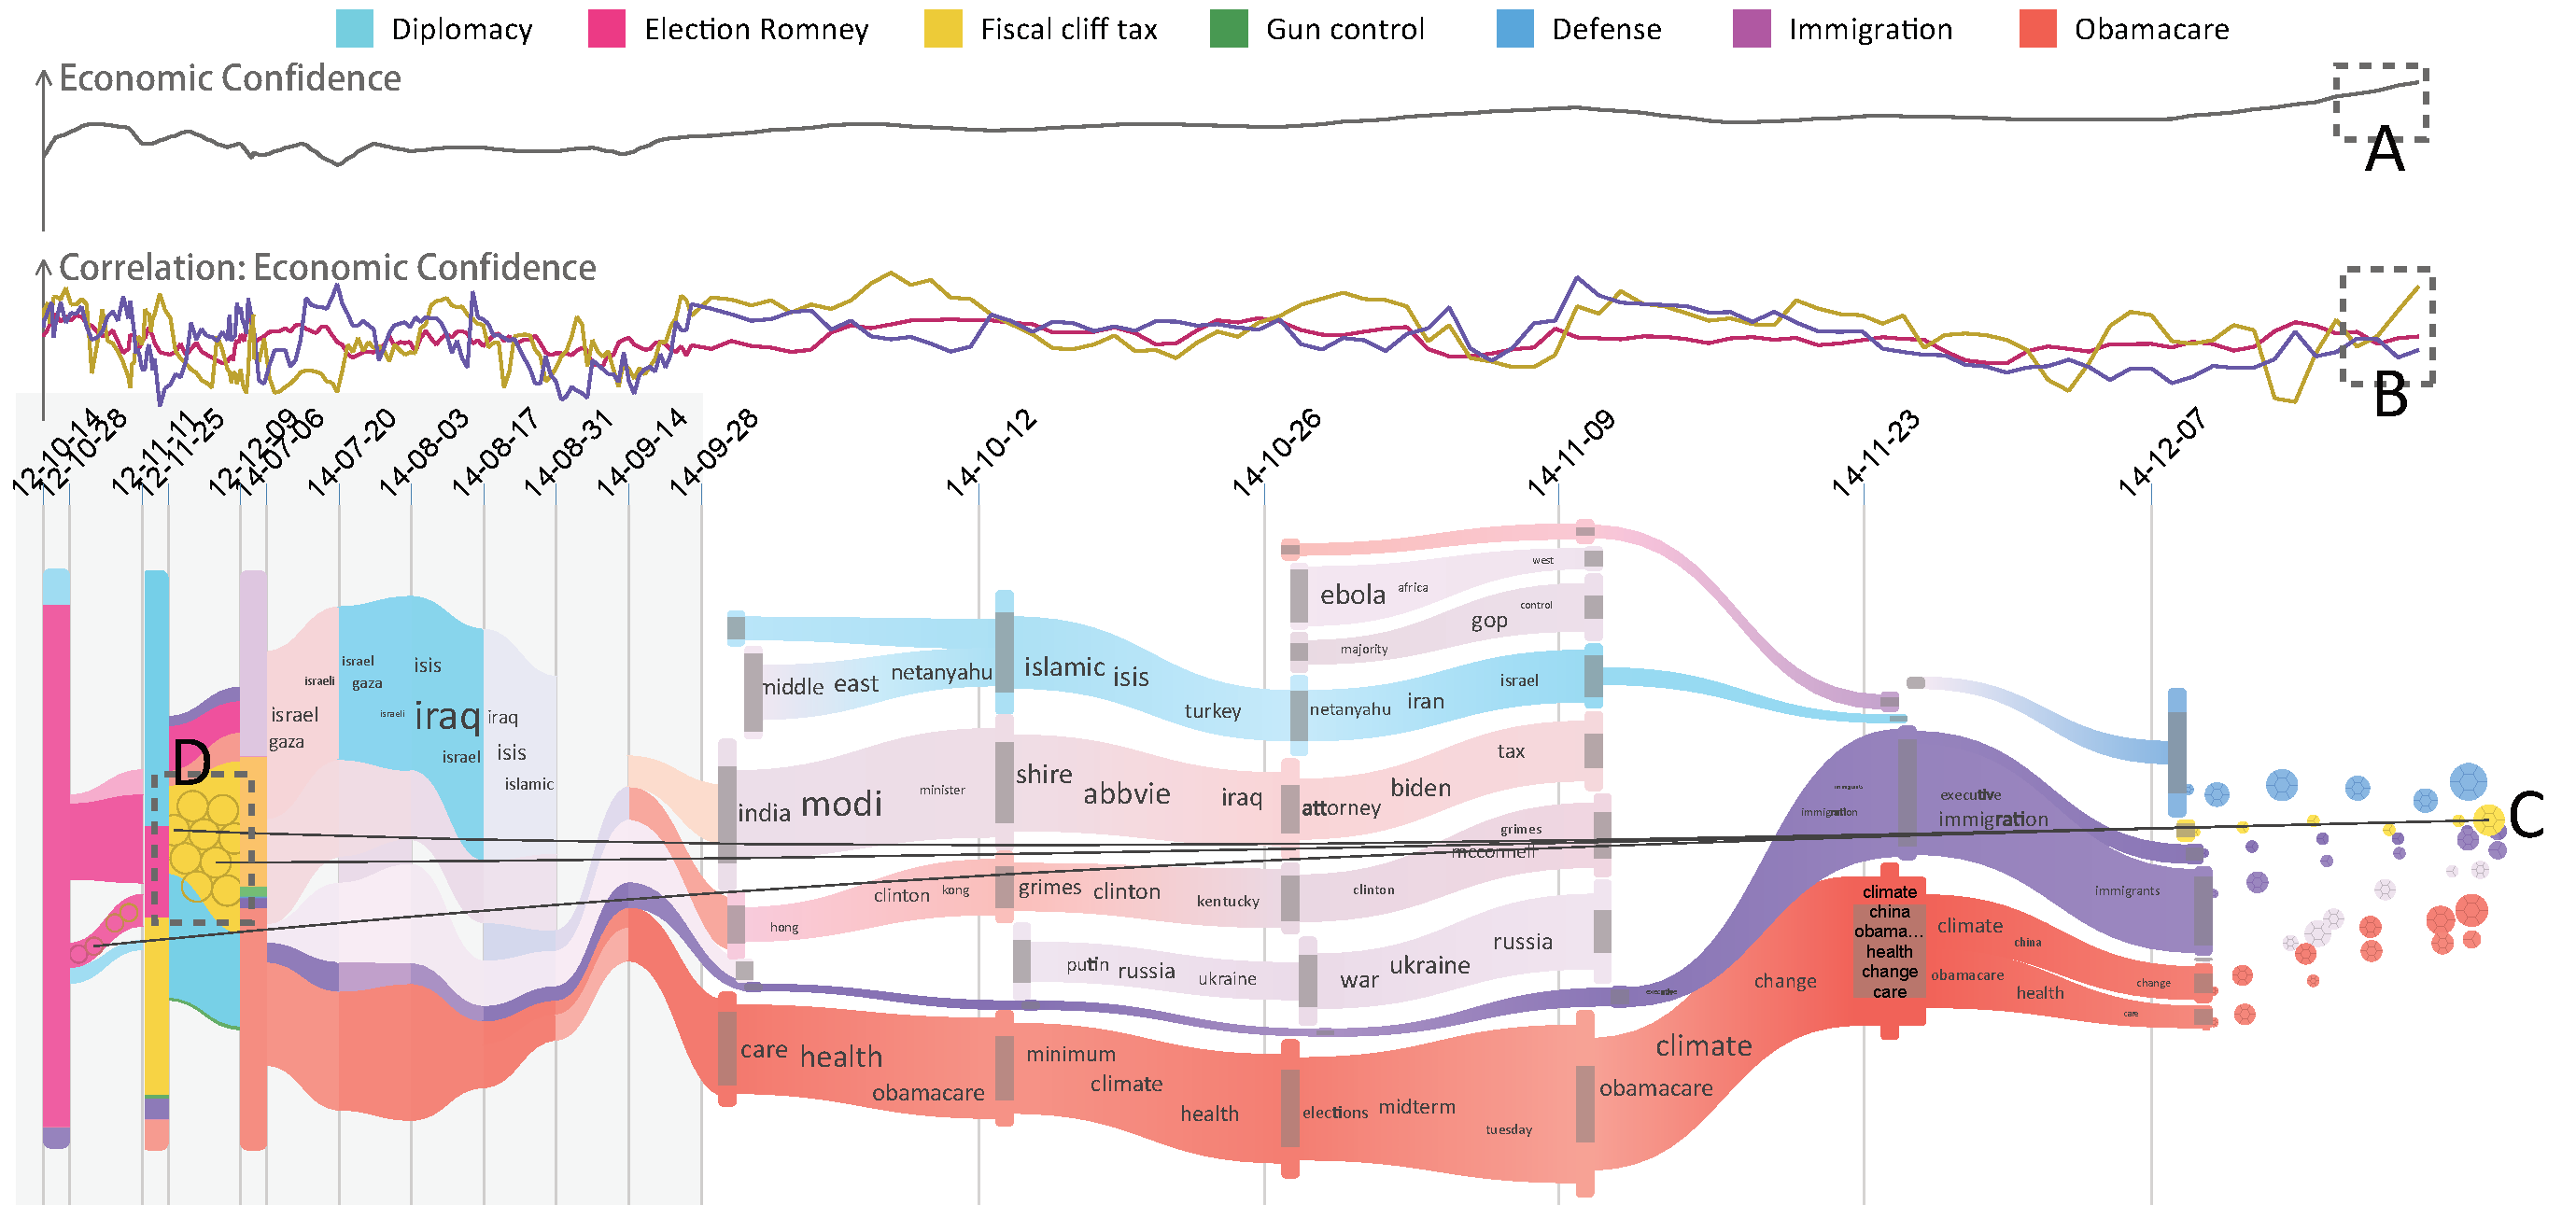
\includegraphics[width=0.85\linewidth]{fig/obamacase2legend}
	\vspace{-2mm}
	\caption{
		%Carry-over effect of the media agenda: the documents about tax raising in 2012 are connected to tax breaks in 2014.
		%Carry-over effect of media agenda: the documents \kg{on} tax \kg{increase} in 2012 are connected to tax breaks in 2014.
		Carry-over effect of media agenda: the documents \kg{on} \docpr{the} tax \kg{increase} in 2012 are connected to tax breaks in 2014.\looseness=-1
	}
	%\vspace{-6mm}
	\label{fig:obamacase2}
	\vspace{-5mm}
\end{figure*}


%After this tragedy people were eager to see tighter gun control (``Gun control petition attracts record interest in US'').
%Obama's action was also in line with public opinion (``Obama's call for action against gun violence''). To see the response of the public to Obama's action professor P1 split the topic and see two major subtopics (Fig.~\ref{fig:obamacase1}G). One subtopic is about Obama's response to the shooting accident (``'')
%This may be one of the leading factors of this increase of the job approval.


%\noindent \textbf{Public attention transited to topic ``Fiscal Cliff.''}
%\noindent \textbf{P ublic attention transited to topic ``\kg{fiscal cliff and taxes}.''}
\noindent \textbf{\normalsize Public attention \dc{transition} to topic ``\kg{fiscal cliff and taxes}.''}
%\textbf{Public approval and public attention transition:}
%Professor (P1) observed an immediate decrease of the precedential approval on Dec. 29, 2012 (Fig.~\ref{fig:obamacase1}D).
%\kg{P1} observed an immediate decrease of the \kg{presidential} approval on Dec. 29, 2012 (Fig.~\ref{fig:obamacase1}D).
%\kg{P1} observed an immediate decrease \dc{in} \kg{presidential} approval on Dec. 31, 2012 (Fig.~\ref{fig:obamacase1}D).
\kg{P1} observed an immediate decrease \dc{in} \docpr{the \kg{presidential} approval rating} on Dec. 31, 2012 (Fig.~\ref{fig:obamacase1}D).
%He was curious about what caused this change.
%The correlation between the precedential approval and topic ``gun control'' decreased to a smaller value (0.12), while its correlation with topic ``fiscal cliff and tax'' increased to the highest (0.51, Fig.~\ref{fig:obamacase1}E).
%The correlation between the \kg{presidential} approval and topic ``gun control'' decreased to a smaller value (0.12), \kg{whereas} its correlation with \kg{the} topic ``fiscal cliff and taxes'' increased to the highest (0.51, Fig.~\ref{fig:obamacase1}E).
The correlation between \dc{presidential} approval and \docpr{the} topic ``gun control'' decreased to a smaller value (0.12), \kg{whereas} its correlation with topic ``fiscal cliff and taxes'' increased to \dc{its} highest (0.51, Fig.~\ref{fig:obamacase1}E).
%After getting a closer look at the ``Fiscal Cliff'' topic,
%He observed that there is a boost of this topic at this time (Fig.~\ref{fig:obamacase1}F).
%Professor P1 commented that this change may be caused by the transition of the public attention to topic ``fiscal cliff and tax.''
%P1 commented that this change \kg{might have been} caused by the transition of the public attention to topic ``fiscal cliff and taxes.''
%P1 \dc{surmised} that this change \kg{might have been} caused by the transition \dc{in} public attention to topic ``fiscal cliff and taxes.''
%This made him more believe that it was the reason.
%He further explained that this topic was talking about the fiscal cliff crisis at the end of 2012.
\kg{P1} explained that this topic was \kg{about} the fiscal cliff crisis at the end of 2012.
%The government was faced with an act taking effect on Jan. 1, 2013.
The government \kg{faced} an act \kg{that would take} effect on Jan. 1, 2013.
%A large tax raising and spending cuts were included in this act.
\kg{Large} tax \kg{increases} and spending cuts were included in this act.
%To postpone this act, the president and the two parties went through a long debate and came to a temporary solution on Jan. 1, 2013.
%To postpone this act, the president and the two \kg{political} parties \kg{debated long and settled with a} temporary solution on Jan. 1, 2013.
To postpone this act, the president and the two \kg{political} parties debated \dc{for a long time} and settled \dc{on} a temporary solution on Jan. 1.
They agreed to postpone the spending cuts until Mar. 1.
%However he did not know what flaws Obama made in handling the crisis which resulted in the critics to him as a president.
%After reading the news he found that people criticized that Obama did not actually want to end this crisis (``Barack Obama and Harry Reid continue their melodramatic playacting, pretending they actually want to stop our nation from going over Obama's Fiscal Cliff'').
%After reading the news\kg{, P1} found that \kg{the public} criticized Obama \kg{for} not actually want to end \kg{the said} crisis (``Barack Obama and Harry Reid continue their melodramatic playacting, pretending they actually want to stop our nation from going over Obama's Fiscal Cliff'').
After reading the news\kg{, P1} found that people \dc{surmised that the president did not truly want the crisis to end}.
 %(``Obama and Reid Continue Playacting'').
%As this topic was about economy, professor P1 switched to the economic confidence index.
%As this topic was \kg{on the} economy, P1 \dc{considered} the economic confidence index.
%As this topic \dc{concerned} economy, P1 \dc{considered} the economic confidence index.
As this topic \dc{concerned} \docpr{the} economy, P1 \dc{considered} the economic confidence index.
%Unsurprisingly, he found a local minimum on Dec. 31, 2012 \kg{(Fig.~\ref{fig:obamacase1}F)}.
Unsurprisingly, a local minimum on Dec. 31, 2012 \kg{(Fig.~\ref{fig:obamacase1}F)} \kg{was found}.
%Because the correlation between this topic and the economic confidence was the highest \kg{(Fig.~\ref{fig:obamacase1}G)},
%The low confidence was possibly caused by raising tax.
%The low confidence \kg{level} was possibly caused by raising tax \kg{rates} \kg{because} the correlation between this topic and the economic confidence was the highest \kg{(Fig.~\ref{fig:obamacase1}G)}.\looseness=-1
The low confidence \kg{level} was possibly caused by raising tax \kg{rates} \kg{because} the correlation between this topic and the economic confidence was \docpr{at its} highest \kg{(Fig.~\ref{fig:obamacase1}G)}.\looseness=-1

%This is consistent with the expert's domain knowledge.

%As the spending cuts of the act was was postponed to Mar. 1, 2013, the professor decided to continue tracking this event.
%As the spending cuts of the act was postponed to Mar. 1, 2013, \kg{P1} decided to continue tracking this event.
As the spending cuts \dc{were} postponed to Mar. 1, \kg{P1} decided to continue tracking this event.
%In the news he learned that this act would have a huge effect on the economy (``Obama said the automatic cuts, known as the sequester, would do great damage to the economy'').
%\kg{Through} the news\kg{,} \kg{P1} learned that this act would have a \kg{significant} effect on the economy (``Bernanke: sequester cuts slow economic recovery'')
He learned that this act would have a \kg{significant} effect on the economy (``Bernanke: sequester cuts slow economic recovery'').
%He found that after two months of negotiation, the two parties did not reach an agreement.
%\kg{and} after two months of negotiation, the two parties \kg{had reached no} agreement.
The spending cuts took effect on Mar. 1.
%On Mar. 1, 2013, he observed another local minimum of the economic confidence \kg{(Fig.~\ref{fig:obamacase1}I)}.
%On \kg{this date}, \kg{P1} observed another local minimum of the economic confidence \kg{(Fig.~\ref{fig:obamacase1}I)}.
On \kg{this date}, \kg{P1} observed another local minimum \dc{in} the economic confidence \kg{(Fig.~\ref{fig:obamacase1}I)}.
%The correlation between the economic confidence and topic ``fiscal cliff and taxes" was the highest \kg{(Fig.~\ref{fig:obamacase1}J)},
%The correlation between the economic confidence and topic ``fiscal cliff and taxes" was \dc{at its} highest \kg{(Fig.~\ref{fig:obamacase1}J)},
The correlation between the economic confidence and \docpr{the} topic ``fiscal cliff and taxes" was \dc{at its} highest \kg{(Fig.~\ref{fig:obamacase1}J)},
%which is in line with the expert's expectation.
which \kg{was} in \kg{accordance} with P1's expectation.
%which was not out of the expert's expectation.
%Professor P1 commented that the streaming visualization is visually appealing and friendly.
%He can use it to examine real-time documents.
%In addition, he can easily tracking the progress of an event and perform analysis to gain insight.
He commented that the streaming visualization \kg{was} visually appealing and practically useful  %shixia to examine
\kg{for examining} real-time documents.\looseness=-1
%\kg{because} tracking the progress of an event and \kg{performing} analysis to gain insight \kg{were easy}.
%\kg{because} tracking the progress of an event and \kg{performing} analysis to gain \dc{insights} \kg{were easy}.

\noindent \textbf{\normalsize Carry-over effect of topic ``fiscal cliff and taxes.''}
%\textbf{Public approval and carry over effect:}
%The case above drew great interest of professor P1.
%professor P1 wanted to follow the subsequent development of this topic.
P1 wanted to follow the subsequent development of this topic.
%He found that topic ``fiscal cliff and tax" (yellow) appeared again on Dec. 21, 2014 (Fig.~\ref{fig:obamacase2}).
%He found that topic ``fiscal cliff and tax" (yellow) appeared again on Dec. 7, 2014 (Fig.~\ref{fig:obamacase2}).
%He found that topic ``fiscal cliff and taxes" (yellow) appeared again on Dec. 7, 2014 (Fig.~\ref{fig:obamacase2}).
%He found that topic ``fiscal cliff and taxes" (yellow) appeared again on Dec. 7, 2014 (Fig.~\ref{fig:obamacase2}).
He found that \docpr{the} topic ``fiscal cliff and taxes" (yellow) appeared again on Dec. 7, 2014 (Fig.~\ref{fig:obamacase2}).
%This topic talked about tax breaks at the end of 2014. %for retailers and teachers
%This topic \kg{focused on} tax breaks at the end of 2014. %for retailers and teachers
This topic \dc{concerned} tax breaks at the end of 2014. %for retailers and teachers
%At this time, the economic confidence index had a remarkable increase (Fig.~\ref{fig:obamacase2}A).
%At this time, the economic confidence index \kg{showed} a remarkable increase (Fig.~\ref{fig:obamacase2}A).
At this time, the economic confidence index \dc{experienced} a remarkable increase (Fig.~\ref{fig:obamacase2}A).
%Because the correlation between this index and topic ``fiscal cliff and tax" was the highest (0.44, Fig.~\ref{fig:obamacase2}B), P1 speculated that intensive discussions on tax breaks in this topic is a potential reason.
%Because the correlation between this index and topic ``fiscal cliff and taxes" was the highest (0.44, Fig.~\ref{fig:obamacase2}B), P1 speculated that \dc{intense} discussions on tax breaks \dc{concerning} this topic \dc{were} a potential reason.
Because the correlation between this index and \docpr{the} topic ``fiscal cliff and taxes" was \docpr{at its} highest (0.44, Fig.~\ref{fig:obamacase2}B), P1 speculated that \dc{intense} discussions on tax breaks \dc{concerning} this topic \dc{were} a potential reason.
%P1 speculated that \kg{the} topic \kg{on tax breaks} \kg{was} a potential reason \kg{for the high} correlation \kg{of the} topic ``fiscal cliff and taxes" (0.44, Fig.~\ref{fig:obamacase2}B).
%P1 was curious why such a small topic had a significant influence on the economic confidence.
\kg{P1} was curious \kg{about the} significant influence \kg{of this small topic} on economic confidence.
%To this end, he linked the largest document cluster (Fig.~\ref{fig:obamacase2}C) at this time to the previous relevant documents.
To this end, \kg{P1} linked the largest document cluster (Fig.~\ref{fig:obamacase2}C) at this time to the previous relevant documents.
%There are several documents appeared during the period of fiscal cliff crisis in 2012 (Fig.~\ref{fig:obamacase2}D).
\kg{Several} documents appeared during the period of \kg{the} fiscal cliff crisis in 2012 (Fig.~\ref{fig:obamacase2}D).
%At that time, the government wanted to raise tax due to fiscal cliff and this topic was the dominant topic in media (the yellow topic in Fig.~\ref{fig:obamacase2}(a) and (b)).
At that time, the government wanted to raise \kg{taxes because of the} fiscal cliff and this topic was dominant in \kg{the} media (yellow topic in Figs.~\ref{fig:obamacase1}(a) and (b)).
%It caused a decrease of the economic confidence.
%Professor P1 commented that this can be regarded as the carry-over effect \cite{carry-over} in his field.
%\kg{P1} commented that this \kg{fact} \kg{could} be regarded as the carry-over effect \cite{carry-over} in \kg{the field of media and communication}.
\kg{P1} commented that this \kg{fact} \kg{could} be regarded as \dc{a} carry-over effect \cite{carry-over} in the field of media and \dc{communication}.
%He further explained, ``The fiscal cliff crisis left a profound impression on the public and had a great influence to the economic confidence at that time.
\kg{P1} further explained, ``The fiscal cliff crisis left a profound impression on the public and had a great influence \kg{on} the economic confidence at that time.
As a result, this influence can be carried over to the relevant topic later even if it is a smaller one.''

%However he was suspicious that this effect could be carried over to two years later.
%To make his analysis complete,

%To verify his assumption that topic ``fiscal cliff and tax" was the major reason, the professor wanted to .
%To find or exclude other possible reasons, the professor continued to check other topics (``defense'' and ``immigration'') occurred during that time.
%To find or exclude other possible reasons, \kg{P1 checked} other topics (``defense'' and ``immigration'') \kg{during that period.}
%%The correlation between the economic confidence and these topics are low (``defense:'' 0.10; ``immigration:'' -0.07).
%%The correlation between the economic confidence and these topics \kg{were} low (``defense:'' 0.10; ``immigration:'' -0.07).
%The correlation between the economic confidence and these topics \dc{was} low (``defense:'' 0.10; ``immigration:'' -0.07).
%%He then excluded these two topics from possible reasons.
%%\kg{P1} then excluded these two topics from \kg{being} possible reasons.
%He then excluded these two topics from being possible reasons.
%%In the visualization, he found another large topic that he did not pay attention to before, ``Obamacare'' (purple).
%In the visualization, \kg{P1} found another large topic \kg{that was previously missed,} ``Obamacare'' (red).
%He added this topic to the focus list and regenerated the visualization.
%%\kg{This} topic \kg{was added} to the focus list and regenerated the visualization.
%%He checked the correlation between topic ``Obamacare'' and the economic confidence and found the correlation is low (0.20).
%\kg{The} correlation between ``Obamacare'' and economic confidence \kg{was} low (0.20).
%%Thus he also excluded this topic.
%Thus\kg{,} this topic \kg{was also excluded.}
%%Finally, the expert concluded that tax breaks may be the leading cause of the economic confidence increase.
%%Finally, the expert concluded that tax breaks \kg{might} be the leading cause of the economic confidence increase.
%\kg{This led to the conclusion that tax breaks were potentially the leading cause for the increase in economic confidence.\looseness=-1}
%Professor P1 was very surprised that the carry-over effect could be such strong that even after two years the topic could still have such a strong influence on the economic confidence.

%444,432 news articles that contain the keyword ``Obama,'' were collected from Sep. 1, 2012 to Jan. 14, 2013.
%Grouped by week, the articles were organized into 18 topic trees. %(Fig.~\ref{fig:obamatree}).
%%The average number of the first level nodes is 41, and the tree depth is 5($\pm 1$).
%The tree depths varied from 4 to 5, the total node numbers changed from 144 to 297, and the node
%number of the first level ranged from 18 to 79.
%
%To provide an overview of the news data to users, our system automatically extracted several initial focus nodes that can suitably represent the dataset and are distinct from one another.
%In our implementation, a clustering method, the mean-shift algorithm, was utilized to cluster the topic at the first level because it is the most abstract level and can represent the topic tree very well.
%Four clusters were detected in the Obama data.
%For each cluster, we selected the node closest to the cluster center as a focus node.
%Four focus nodes were automatically derived to generate the default overview (Fig.~\ref{fig:obama}(a)).
%In the overview, the four colors represent four different topics: ``Iran'' (red), ``Tax'' (yellow), ``Debate'' (green), and ``Gun Control'' (purple).
%As shown in Fig.~\ref{fig:obama}(a), significant variations existed; however, some overall patterns clearly stood out.
%The green and yellow topics were dominant and divided the entire time period into two parts.
%The red topic was small but persistent and the purple one was large but irruptive.
%
%In the first half of the time period (before Nov. 3), the ``Debate'' (green) topic dominated and unsurprisingly ended in the week of Nov. 6, 2012, the date when Obama was reelected as president.
%In addition, the ``Tax'' (yellow) topic was partially related to the ``Debate'' (green) topic from time to time.
%Initially, the yellowish green topic (marked as \textbf{A} in Fig.~\ref{fig:obama}(a)), a mixed topic of ``Debate'' and ``Tax,'' merged with the green one.
%This merging was caused by the tax-related debates (``Obama, Romney Clash on Economy, Taxes in First Debate'').
%The yellowish green topic gradually split from the green one because its focus shifted to the economy, jobs, and the fiscal cliff.
%If users are interested in tracking the mixed topic, they could interactively split the topic nodes and extract them from the green topic (Fig.~\ref{fig:obama}(b)).
%
%
%Similarly, the ``Iran'' (red) topic  interacted with the ``Debate'' (green) topic in the week of Oct. 20 (marked as \textbf{B} in Fig.~\ref{fig:obama}(a)).
%After splitting the topic nodes into small ones (Fig.~\ref{fig:obama}(c)), a red topic node that contained several news articles on ``Iran'' was observed
%For example, one of them is ``Obama, Romney on Israel and Iran.'' This article clearly indicates why these two topics merged.
%
%After the week of Nov. 3 (the second half of the time period), the ``Tax'' (yellow) topic dominated the view.
%Considering that it has fewer connections with other topics, it was more isolated than the ``Debate'' topic.
%Within these topics, the yellow nodes were almost fully connected with one another; thus, the ``Tax'' was also a relatively stable topic.
%
%Although the ``Tax'' (yellow) topic was dominant during this time period, two greenish nodes (marked as \textbf{C} and \textbf{D} in Fig.~\ref{fig:obama}(a)) still appeared.
%Clearly, these two topics have different evolution patterns.
%Judging from the connections between \textbf{C} and the other nodes, \textbf{C} was likely a momentary topic.
%To verify this hypothesis, we examined \textbf{C}'s content and found that it was focused on ``Romney blames loss on Obama's `gifts' to voters,'' which was indeed a momentary event.
%On the other hand, \textbf{D} was fully connected to the yellow nodes. This connection indicates \textbf{D} contains news articles related to both the ``Debate'' and ``Tax'' topics. For example, one of the articles had the title ``GOP fights President Barack Obama on his campaign promise to raise taxes on the rich.''\looseness=-1
%
%
%The ``Gun Control'' (purple) topic, which was caused by the Connecticut Elementary School massacre on Dec. 14, 2012, was then explored.
%The event caused a topic burst in the week of Dec. 15.
%Its horizontal offset indicates that it is a high-level topic node.
%%Although the topic has a burst in the week of December 15, our system still finds several related topics, colored in purple, before the burst (marked as dotted rectangles in Fig.~\ref{fig:obama}(a)).
%%Since they are highly related to our focus node, they are still successfully separated from the others.
%%For example, in the week of Dec. 1, 2012 (marked as \textbf{E}), a node of only five documents talks about ``Obama to Push Gun Control in Second Term?''.
%Then we split the big purple node and checked the two smaller topics in it (Fig.~\ref{fig:obama}(d)).
%The lower node was mainly about the public discussion on gun control.
%The strong connection of this node to the topic on the right indicates that it was still the major topic at the next time point.
%When the node was split further, more detailed topics revealed themselves (Fig.~\ref{fig:obama}(e)).
%From top to bottom, these topics were ``NRA calls for armed guards at every school,'' ``Obama turns to Biden on gun control measures,'' ``Guns fly off shelves,'' ``Assault weapons ban,'' and ``Connecticut school shooting: how to talk to your kids'' (marked as \textbf{F} to \textbf{J}, respectively).
%The upper node, which represents follow-up news to the tragedy, has weaker connections to the right.
%This condition indicates that the topic shrunk considerably at the next time point.

%  \vspace{-4mm}

%\begin{figure}[t]
%  \centering
%  \includegraphics[width=\columnwidth]{fig/2clintonoverview}
%    \vspace{-4mm}
%  \caption{
%%  \small
%  Topics related to ``Bill Clinton'' and ``Hillary Clinton.''\looseness=-1}
%  \vspace{-3mm}
%  \label{fig:2clintonoverview}
%\end{figure}



%from Shixia, the below story can be deleted if the qualitative evaluation need more space.



%The search function can help users explore more specific topics.
%For example, we entered ``Clinton'' in the search box.
%The first topic node recommended by our system is about the speech at the Democratic National Convention on Sep. 5, 2012.
%We selected it as the focus node and visualized the result.
%As shown in Fig.~\ref{fig:clintonoverview}, the topic was only active in the first week (marked as \textbf{A}).
%However, in the week of Oct. 20, a small but highly related topic node appeared (marked as \textbf{B}).
%We clicked it to see the detailed content and found that it contained two sub-topic nodes: ``Bill Clinton to rally for Obama at Springs Preserve'' and ``Hillary Clinton says she's `unlikely' to stay Secretary of State'' (marked as \textbf{C}).
%To further explore these nodes, we regarded both nodes as new focus nodes and transformed the visualization.
%Fig.~\ref{fig:2clintonoverview} shows that the two Clintons mainly have one overlapping topic (marked as \textbf{D}), which is ``Bill Clinton's DNC speech: Setting the stage for Hillary in 2016?''
%
%%In the middle of Fig.~\ref{fig:2clintonoverview}, our tree cut algorithm successfully splits the context topic and reveals two small relevant topics hidden inside, which are a discussion about ``Poll: Clinton favored in 2016 in Iowa''.
%
%The topics on Hillary Clinton in the top of Fig.~\ref{fig:2clintonoverview} can be  divided into two parts (marked by \textbf{F} and \textbf{G}).
%\textbf{F} is about the Libya Attack, in which Hillary Clinton was highly involved.
%In the week of Oct. 13, the article with the title ``Hillary Clinton Takes Blame for Benghazi Attack'' ended that topic (marked by \textbf{E}).
%\textbf{G} contains two separate topics related to Hillary Clinton whose colors indicate that one is more relevant to the focus than the other.
%In fact, the greener one is about Hillary Clinton herself.
%For example, two articles have the titles ``Clinton is the people's choice for 2016 Prez bid: Poll,'' and ``Obama calls Clinton to wish her well as she recovers from concussion.''
%However, the other is about the secretary of state candidates, in which Hillary Clinton is partially involved.



